
\section{Ensemble de données}
\paragraph{}
Afin de développer le module d'apprentissage automatique mentionné dans précédemment (voir \ref{ProlemSolver}), nous avons choisit le data-set\footnote{Ensemble de données d'apprentissage} disponible dans \cite{dataset}, il s'agira donc d'analyser ces données, de les pré-traiter éventuellement afin de les préparer pour la session d'apprentissage CITER FUCKING  LEARNING HEEEEEERRE
\subsection{Description des données}
\paragraph{}
Comme expliqué dans \cite{datasetDetails}, les données d'apprentissage on été récupéré a l'aide l'application Vicon-Tracker \cite{vico} ainsi que celle de marqueurs(au total de 11) placés sur la face arrière d'un gant, ces derniers servent de source de données envoyé à des capteurs positionnés sur les deux flancs(pour calculer la profondeur), la figure suivante illustre le procédé : 
\begin{minipage}{0.5\linewidth}
	\begin{figure}[H]
		\centering
		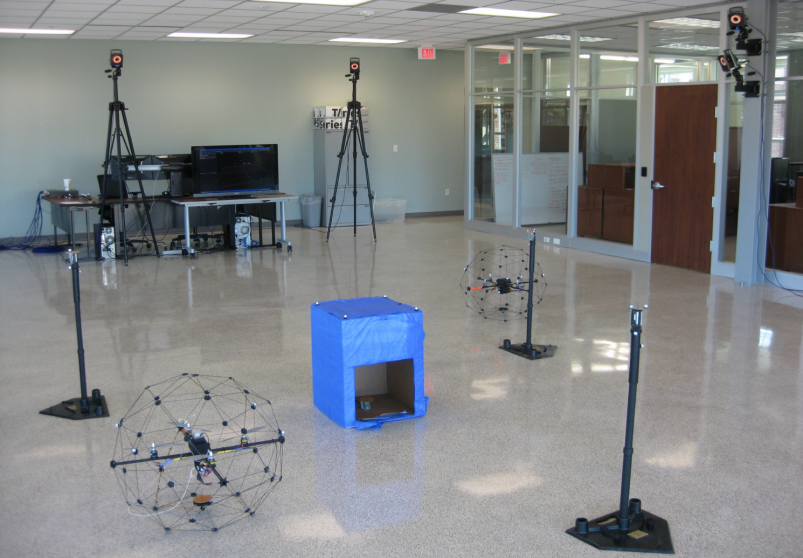
\includegraphics[width=\linewidth]{images/cameras.png}
		\caption{\small Environement ou les données on été capturées \cite{datasetDetails}}
	\end{figure}
\end{minipage}
\begin{minipage}{0.5\linewidth}
	\begin{figure}[H]
		\centering
		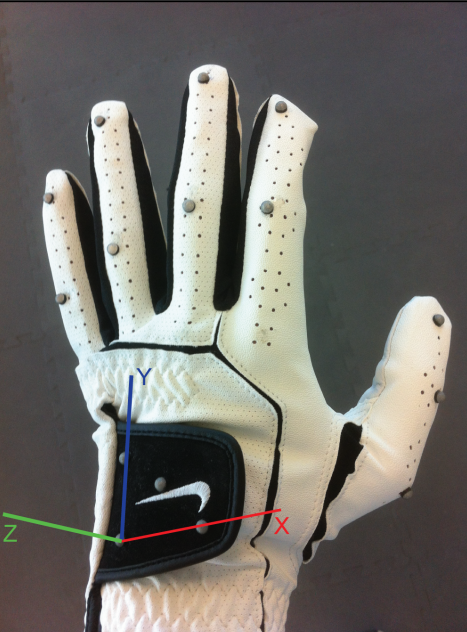
\includegraphics[width=0.5\linewidth]{images/glove.png}
		\caption{\small  Le gant utilisé pour y attaché les marqueurs( la source des données ) \cite{datasetDetails}}
	\end{figure}
\end{minipage}
\par 
Dans \cite{dataset}, on peut notamment trouvé une brève description des données brutes, elles sont sous forme d'un fichier \textbf{.csv} avec le délimiteur de cellules \textbf{,} (virgule), l'entête est structurée  de la manière suivante :
\begin{itemize}
	\item Les deux premières colonnes Class/User représentent répsectivement l'identifiant du geste observé (1 à 5) et l'identifiant de l'utilisateur(cobaye) qui a porté le gant durant cette session de collecte de données.
	\item Les 36 colonnes suivantes contiennent des nombres réels qui représentent les coordonnées cartésiennes en 3-dimensions $(x_i,y_i,z_i)$ des différents marqueurs $Marker_i$. \par Il est a noté d'après \cite{datasetDetails} et \cite{dataset} que les marqueurs sont non-étiquetés, c'est à dire que pour deux instances $I_1 et I_2$ du data-set, les coordonnés $(x_i^{I_1},y_i^{I_1},z_i^{I_1})$ et $(x_i^{I_2},y_i^{I_2},z_i^{I_2})$ ne désignent pas toujours les coordonnées du même marqueurs $i$. \par En raison des conditions de captage des données certaines instances ont des données manquantes représentées par \textbf{?}
\end{itemize}
\subsection{Analyse et prétraitement des données}
\paragraph{}
Une étape primordiale avant de se lancer dans les essaies d'apprentissage est l'analyse et la codification des données, nous avons d'abord effectué une analyse manuelle pour essayer de comprendre comment les données variaient, en nous inspirant des remarques faites dans \cite{datasetDetails} nous avons remarqué ce qui suit : 
\begin{itemize}
	\item Les instances qui disposent de données manquantes ont au minimum 	
\end{itemize}
\subsubsection{Approche naïve}
\paragraph{}
\subsubsection{Approche par Clustering}
\paragraph{}